\part{基本服务篇}

本章介绍几种常见的服务。这里不注重概念的介绍,概念只做简短的描述,主要
介绍如何实施及实现这些服务。

\chapter{DHCP}

动态主机配置协议(DHCP)\index{DHCP},

\begin{enumerate}[itemsep=0pt,parsep=0pt]
\item 服务端端口67/UDP
\item 客户端端口68/UDP
\item 客户端发送DHCPDISCOVER在网络中寻求地址分配
\item 服务端回应DHCPDISCOVER请求
\item 客户端发送DHCPREQUEST
\item 服务端发送DHCPACK
\item 客户端得到地址
\end{enumerate}

主配 cp /usr/share/doc/dhcp-<version>/dhcpd.conf.sample /etc/dhcpd.conf
包含以下7项 服务器即可搭建

\small{
\begin{verbatim}
1. ddns-update-style
2. subnet
3. option
4. range dynamic-bootp
5. default-lease-time
6. max-lease-time
7. host
\end{verbatim}
}
\normalsize

\small{
\begin{verbatim}
ddns-update-style interim;
ignore client-updates;
default-lease-time 600;
max-lease-time 7200;

subnet 192.168.0.0 netmask 255.255.255.0 {
    next-server 192.168.0.128;
    filename="pxelinux.0";
    option routers 192.168.0.128;
    option subnet-mask 255.255.255.0;
    option nis-domain "lavenliu.com";
    option domain-name "lavenliu.com";
    option ntp-servers 192.168.0.254;
    range dynamic-bootp 192.168.0.100 192.168.0.130;
    host stu1 {
      next-server lavenliu.com;
      hardware Ethernet 12:34:56:78:AB:CD;
      fixed-address 192.168.0.2;
    }
}
\end{verbatim}
}
\normalsize

\chapter{FTP}

\chapter{NFS}

NFS(Network File System)\index{NFS}网络文件系统,目前依然非常流行。
NFS的一个最大优点是具有广泛的支持:大部分的类UNIX都可以支持NFS。NFS通常
比其他的网络文件系统更容易配置和使用。与其他网络文件系统一样,NFS可以在
服务器或任何一个客户端上修改文件,然后在其他所有系统上可以立即使用修改
后的文件。

\section{配置NFS服务器}

\section{配置NFS客户端}

\chapter{Kickstart}

Red Hat Linux提供了一种非常方便的自动化系统安装方式,即为
kickstart\index{kickstart}。这种工具的出现,极大的方便了众多的系统管理
员或装机攻城狮。有了它,我们就不用拿着光盘或U盘在机房来回乱窜地装机了,
我们可以在办公室通过IPMI的方式来操作。不管这个工具有多优秀,相比之前单
台的安装方式,效率提升了很多。当然,也有另外几种较优越的自动化系统安装
工具,这里就不介绍了。

kickstart文件包含了安装程序所使用的指令,在安装的过程中可以用来减少或者
消除用户输入的麻烦。

在系统数目巨大且完全相同的时候,kickstart文件非常有用。


\begin{figure}[htbp]
  \begin{center}
    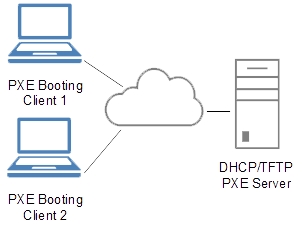
\includegraphics[width=.5\textwidth]{graph/PXE_diagram.png}
  \end{center}
  \caption{PXE WorkFlow}
  \label{fig:pxeWork}
\end{figure}

PXE工作流程图:
\begin{figure}[htbp]
  \begin{center}
    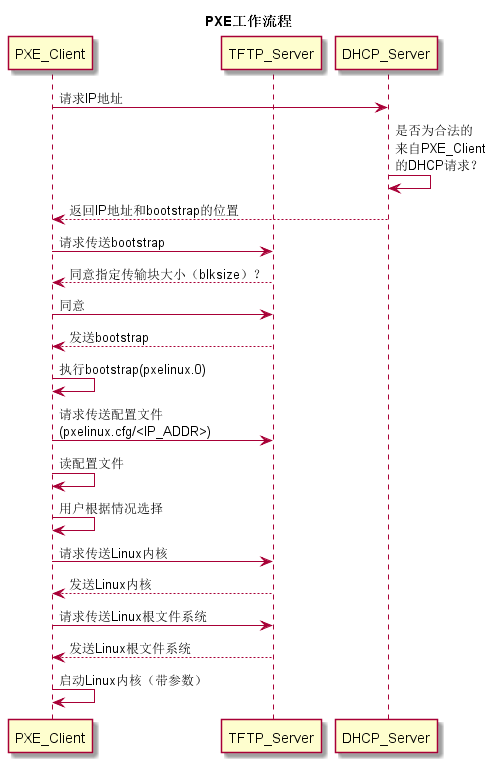
\includegraphics[width=.55\textwidth]{graph/pxe01.png}
  \end{center}
  \caption{PXE工作流程图}
  \label{fig:pxeWorkFlow}
\end{figure}

\section{安装相关软件包}

\small{
\begin{verbatim}
	rpm -ivh dhcpdxxx
	rpm -ivh nfs-utilsxxx
	rpm -ivh tftp-serverxxx
	rpm -ivh xinetdxxx
	rpm -ivh httpdxxx
	rpm -ivh syslinuxxxx
	rpm -ivh system-config-kickstartxxx
\end{verbatim}
}
\normalsize

\small{
\begin{verbatim}
 # chkconfig tftp on
   # chkconfig xinetd on
\end{verbatim}
}
\normalsize
   
3. Stop some services, such as selinux, iptables
   setenforce 0
or  vi /etc/sysconfig/selinux disabled
    service iptables stop

4. Copy the related files to the related path

\small{
\begin{verbatim}
# mount /dev/cdrom /media
# mkdir /var/ftp/pub/RedHat
# cp -a /media/* /var/ftp/pub/RedHat
# cp /usr/share/syslinux/pxelinux.0 /tftpboot
# cp /var/ftp/pub/RedHat/isolinux/vmlinuz /tftpboot
# cp /var/ftp/pub/RedHat/isolinux/initrd.img /tftpboot
# mkdir /tftpboot/pxelinux.cfg
# vi /tftpboot/pxelinux.cfg/default 
     default install
     prompt 1
     timeout 60
     label local
	localhost	1
     label install
	kernel vmlinuz
	append initrd=initrd.img ramdisk_size=8192 ks=http://192.168.0.254/ks/ks.conf
\end{verbatim}
}
\normalsize

\small{
\begin{verbatim}
   # mount /dev/cdrom /media
   # mkdir /var/ftp/pub/RedHat
   # cp -a /media/* /var/ftp/pub/CentOS
   # cp /usr/share/syslinux/pxelinux.0 /var/lib/tftpboot
   # cp /var/ftp/pub/CentOS/isolinux/vmlinuz /var/lib/tftpboot
   # cp /var/ftp/pub/CentOS/isolinux/initrd.img /var/lib/tftpboot
   # mkdir /var/lib/tftpboot/pxelinux.cfg
   # vi /var/lib/tftpboot/pxelinux.cfg/default
	default install
	prompt 1
	timeout 60
	label local
		localhost	1
	label install
		kernel vmlinuz
		append initrd=initrd.img ramdisk_size=8192 ks=http://192.168.0.254/ks/ks.conf
\end{verbatim}
}
\normalsize

5. Modify the related configure files

\small{
\begin{verbatim}
# vi /etc/dhcp/dhcpd.conf
......
......
next-server	ip_addr;
filename	"pxelinux.0";
......

# vi /etc/http/conf/httpd.conf
Allow from all
# chown -R apache.apache /var/www

# vi /etc/exports
/var/ftp/pub/RedHat 192.168.0.0/255.255.255.0(ro,sync)
\end{verbatim}
}
\normalsize

6. Start services, and later the client can install OS

\small{
\begin{verbatim}
   # service xinetd restart
   # service nfs restart
   # service vsftpd restart
   # service httpd restart
   # service dhcpd restart
\end{verbatim}
}
\normalsize

NOTE:
In the ks.cfg, the keyword 
clearpart --none is default
change this into:
clearpart --all

\chapter{Samba}

\chapter{LAMP}

\section{安装依赖包}

Needless to say, you should install required system packages. So you
cancontinue the next steps. :-)

Be sure these packages are installed:

\small{
\begin{verbatim}
  gcc
  gcc-c++
  flex
  bison
  autoconf
  automake
  bzip2-devel
  ncurses-devel
  libjpeg-devel
  libpng-devel
  libtiff-devel
  freetype-devel
  pam-devel
\end{verbatim}
}
\normalsize

\section{安装额外的包}

In this section, we need to compile and install four packages:

\begin{enumerate}[itemsep=0pt,parsep=0pt]
\item GD2
  \small{
\begin{verbatim}
  [root@lamp ~] # cd /usr/local/src
  [root@lamp src] # tar xzvf gd-2.0.34.tar.gz
  [root@lamp src] # cd gd-2.0.34
  [root@lamp gd-2.0.34] # ./configure --prefix=/usr/local/gd2
  [root@lamp gd-2.0.34] # make
  [root@lamp gd-2.0.34] # make install  
\end{verbatim}
  }
  \normalsize

\item LibXML2
  \small{
\begin{verbatim}
  [root@lamp ~] # cd /usr/local/src
  [root@lamp src] # tar xzvf libxml2-2.6.29.tar.gz
  [root@lamp src] # cd libxml2-2.6.29
  [root@lamp libxml2-2.6.29] # ./configure --prefix=/usr/local/libxml2
  [root@lamp libxml2-2.6.29] # make
  [root@lamp libxml2-2.6.29] # make install
\end{verbatim}
  }
  \normalsize

\item LibMcrypt
  \small{
\begin{verbatim}
  [root@lamp ~] # cd /usr/local/src
  [root@lamp src] # tar xjvf libmcrypt-2.5.8.tar.bz2
  [root@lamp src] # cd libmcrypt-2.5.8
  [root@lamp libmcrypt-2.5.8] # ./configure --prefix=/usr/local/libmcrypt
  [root@lamp libmcrypt-2.5.8] # make
  [root@lamp libmcrypt-2.5.8] # make install
\end{verbatim}
  }
  \normalsize

\item OpenSSL
  \small{
\begin{verbatim}
  [root@lamp ~] # cd /usr/local/src
  [root@lamp src] # tar xzvf openssl-0.9.8e.tar.gz
  [root@lamp src] # cd openssl-0.9.8e
  [root@lamp openssl-0.9.8e] # ./config --prefix=/usr/local/openssl
  [root@lamp openssl-0.9.8e] # make
  [root@lamp openssl-0.9.8e] # make test
  [root@lamp openssl-0.9.8e] # make install
\end{verbatim}
  }
  \normalsize

\end{enumerate}

\section{编译安装MySQL}

\small{
\begin{verbatim}
  [root@lamp ~] #tar xzvf mysql-5.0.27.tar.gz
  [root@lamp ~] # cd mysql-5.0.27
  [root@lamp mysql-5.0.27] # ./configure \
  "--prefix=/usr/local/mysql" \
  "--localstatedir=/var/lib/mysql" \
  "--with-mysqld-user=mysql" \
  "--without-debug" \
  "--with-big-tables" \
  "--with-extra-charsets=all" \
  "--with-pthread" \
  "--enable-static" \
  "--enable-thread-safe-client" \
  "--with-client-ldflags=-all-static" \
  "--with-mysqld-ldflags=-all-static" \
  "--enable-assembler" \
  "--without-isam" \
  "--without-innodb" \
  "--without-ndb-debug"
  
  [root@lamp msyql-5.0.27] # make
  [root@lamp mysql-5.0.27] # make install
  [root@lamp mysql-5.0.27] # useradd mysql
  [root@lamp mysql-5.0.27] # cd /usr/local/mysql
  [root@lamp mysql] # bin/mysql_install_db --user=mysql
  [root@lamp mysql] # chown -R root:mysql .
  [root@lamp mysql] # chown -R mysql /var/lib/mysql
  [root@lamp mysql] # cp share/mysql/my-huge.cnf /etc/my.cnf
  [root@lamp mysql] # cp share/mysql/mysql.server /etc/rc.d/init.d/mysqld
  [root@lamp mysql] # chmod 755 /etc/rc.d/init.d/mysqld
  [root@lamp mysql] # chkconfig --add mysqld
  [root@lamp mysql] # chkconfig --level 3 mysqld on
  [root@lamp mysql] # /etc/rc.d/init.d/mysqld start
  [root@lamp mysql] # bin/mysqladmin -u root password 'clear123'
\end{verbatim}
}
\normalsize

\section{编译安装Apache}

\small{
\begin{verbatim}
  [root@lamp src] # cd /usr/local/src
  [root@lamp src] # tar xjvf httpd-2.2.4.tar.bz2
  [root@lamp src] # cd httpd-2.2.4
  [root@lamp httpd-2.2.4] # ./configure \
  "--prefix=/usr/local/apache2" \
  "--with-included-apr" \
  "--enable-so" \
  "--enable-deflate=shared" \
  "--enable-expires=shared" \
  "--enable-rewrite=shared" \
  "--enable-static-support" \
  "--disable-userdir"
  [root@lamp httpd2.2.4] # make
  [root@lamp httpd2.2.4] # make install
  [root@lamp httpd2.2.4] # echo '/usr/local/apache2/bin/apachectl start' \
  > >> /etc/rc.local
\end{verbatim}
}
\normalsize

\section{编译安装PHP}

\small{
\begin{verbatim}
  [root@lamp ~] # cd /usr/local/src
  [root@lamp src] # tar xjvf php-5.2.3.tar.bz2
  [root@lamp php-5.2.3] # cd php-5.2.3
  [root@lamp php-5.2.3] # ./configure \
  "--prefix=/usr/local/php" \
  "--with-apxs2=/usr/local/apache2/bin/apxs" \
  "--with-config-file-path=/usr/local/php/etc" \
  "--with-mysql=/usr/local/mysql" \
  "--with-libxml-dir=/usr/local/libxml2" \
  "--with-gd=/usr/local/gd2" \
  "--with-jpeg-dir" \
  "--with-png-dir" \
  "--with-bz2" \
  "--with-freetype-dir" \
  "--with-iconv-dir" \
  "--with-zlib-dir " \
  "--with-openssl=/usr/local/openssl" \
  "--with-mcrypt=/usr/local/libmcrypt" \
  "--enable-soap" \
  "--enable-gd-native-ttf" \
  "--enable-memory-limit" \
  "--enable-ftp" \
  "--enable-mbstring" \
  "--enable-exif" \
  "--disable-ipv6" \
  "--disable-cgi" \
  "--disable-cli"
  [root@lamp php-5.2.3] # make
  [root@lamp php-5.2.3] # make install
  [root@lamp php-5.2.3] # mkdir /usr/local/php/etc
  [root@lamp php-5.2.3] # cp php.ini-dist /usr/local/php/etc/php.ini
\end{verbatim}
}
\normalsize

\section{安装Zend加速器}

\small{
\begin{verbatim}
  [root@lamp ~]# cd /usr/local/src
  [root@lamp ~]# tar xf ZendOptimizer-3.2.8-linux-glibc21-i386.tar.gz
  [root@lamp ~]# ./ZendOptimizer-3.2.8-linux-glibc21-i386/install.sh
\end{verbatim}
}
\normalsize

\section{整合Apache与PHP}

We should modify configure file httpd.conf:

\small{
\begin{verbatim}
[root@lamp ~]# emacs /usr/local/apache2/conf/httpd.conf
\end{verbatim}
}
\normalsize

Find this line,

\small{
\begin{verbatim}
AddType application/x-gzip .gz .tgz
\end{verbatim}
}
\normalsize

Add on line under this line,

\small{
\begin{verbatim}
AddType application/x-httpd-php .php
\end{verbatim}
}
\normalsize

Find these lines,

\small{
\begin{verbatim}
<IfModule dir_module>
DirectoryIndex index.html
<IfModule>
\end{verbatim}
}
\normalsize

Change them like this,

\small{
\begin{verbatim}
<IfModule dir_module>
DirectoryIndex index.html index.htm index.php
<IfModule>
\end{verbatim}
}
\normalsize

Find these lines and uncomment them,

\small{
\begin{verbatim}
#Include conf/extra/httpd-mpm.conf
#Include conf/extra/httpd-info.conf
#Include conf/extra/httpd-vhosts.conf
#Include conf/extra/httpd-default.conf
\end{verbatim}
}
\normalsize

When finished, save it! Then restart apache service,

\small{
\begin{verbatim}
[root@lamp ~]# /usr/local/apache2/bin/apachectl restart
\end{verbatim}
}
\normalsize

\chapter{多网卡绑定bonding}

Linux bonding提供将多个网络接口设备捆绑为单个网络接口设置来使用,用于网
络负载均衡及网络冗余。

以太网平衡设备即使用两个或两个以上的网络接口模拟一个虚拟的网络接口用以
外部网络连接。这多个真实网络接口可以连接在同一交换设备或多个交换设备上,
以达到多通路高可用性。在所有真实网络接口中可以指定其中某些真实网络接口
活跃,其他真实网络接口在活跃的真实网络接口故障时接管网络传输;也可以指
定所有真实网络接口活跃,分担全部网络传输带宽。
 
通道绑定(Channel bonding)需要服务器至少拥有2个以太网卡,当使用绑定功能
的时候,
 
bonding模块会使用第一个实际网卡的MAC地址来通信,在侦测到这个网卡失败以
后,它会把这个MAC地址指定到另一块网卡上。

\section{bonding的几种模式}

bonding只能提供链路监测,即从主机到交换机的链路是否接通。如果只是交换机
对外的链路down掉了,而交换机本身并没有故障,那么bonding会认为链路没有问
题而继续使用。
 
miimon是用来进行链路监测的。 比如:miimon=100,那么系统每100ms监测一次链
路连接状态,如果有一条线路不通就转入另一条线路;mode的值表示工作模式,
他共有0,1,2,3,4,5,6七种模式,作者遇到的场景是使用的1,0,6三种,
其他场景适合哪些模式作者也不清楚。
 
mode=1,表示fault-tolerance (active-backup)提供网络冗余功能,工作方式是
主备模式,也就是说默认情况下只有一块网卡工作,另一块做备份。
 
mode=0,表示load balancing (round-robin)为负载均衡模式,两块网卡都工作,
但是与网卡相连的交换机必须做特殊配置( 这两个端口应该采取聚合方式),因
为做bonding的这两块网卡是使用同一个MAC地址。
 
mode=6,表示load balancing (round-robin)为负载均衡方式,两块网卡都工作,
但是该模式下无需配置交换机,因为做bonding的这两块网卡是使用不同的MAC地
址。
 
\section{RHEL下配置bonding}

\section{SuSE下配置bonding}

bond0配置:

\small{
\begin{verbatim}
# cat /etc/sysconfig/network/ifcfg-bond0
DEVICE='bond0'
ONBOOT='yes'
BOOTPROTO='static'
IPADDR='0.0.0.0/24'   
STARTMODE='auto'
BONDING_MASTER='yes'
BONDING_MODULE_OPTS='mode=1 miimon=100'
BONDING_SLAVE0='eth0'
BONDING_SLAVE1='eth1'
USERCONTROL='no'
\end{verbatim}
}
\normalsize

br0配置:

\small{
\begin{verbatim}
# cat /etc/sysconfig/network/ifcfg-br0
BOOTPROTO='static'
BRIDGE='yes'
BRIDGE_FORWARDDELAY='0'
BRIDGE_PORTS='bond1'
BRIDGE_STP='off'
IPADDR='0.0.0.0/24'    	##管理网ip
STARTMODE='auto'
USERCONTROL='no'

# cat /etc/sysconfig/network/ifcfg-vlan0     ##为网卡打Vlan Tag
BOOTPROTO='static'
ETHERDEVICE='br0'
IPADDR='145.240.21.11/24'
STARTMODE='auto'
USERCONTROL='no'
VLAN_ID='210'                       ##上联核心交换机端口的Vlan号

# cat /proc/net/vlan/config         ##验证Vlan是否设置成功
VLAN Dev name | VLAN ID
Name-Type: VLAN_NAME_TYPE_RAW_PLUS_VID_NO_PAD
vlan0         | 210 | br0
\end{verbatim}
}
\normalsize

\section{单网卡多IP配置}
\label{sec:SingleCardMultiIP}

\chapter{LVM硬盘管理及扩容}

LVM是 Logical Volume Manager(逻辑卷管理)的简写,它由Heinz Mauelshagen在
Linux 2.4内核上实现。LVM将一个或多个硬盘的分区在逻辑上集合,相当于一个
大硬盘来使用,当硬盘的空间不够使用的时候,可以继续将其它的硬盘的分区加
入其 中,这样可以实现磁盘空间的动态管理,相对于普通的磁盘分区有很大的灵
活性。
 
与传统的磁盘与分区相比,LVM为计算机提供了更高层次的 磁盘存储。它使系统
管理员可以更方便的为应用与用户分配存储空间。在LVM管理下的存储卷可以按需
要随时改变大小与移除(可能需对文件系统工具进行升 级)。LVM也允许按用户组
对存储卷进行管理,允许管理员用更直观的名称(如"sales'、 'development')代
替物理磁盘名(如'sda'、'sdb')来标识存储卷。
 
如图所示LVM模型:
 
由四个磁盘分区可以组成一个很大的空间,然后在这些空间上划分一些逻辑分区,
当一个逻辑分区的空间不够用的时候,可以从剩余空间上划分一些空间给空间不
够用的分区使用。

\chapter{使用U盘安装Gnu系统}

使用U盘安装系统在某些时候还是很方便的,其安装速度也是蛮给力的。

\section{准备工作}

\begin{enumerate}[itemsep=0pt,parsep=0pt]
\item 4G以上的优盘,格式化成FAT32
\item 镜像编辑软件UltraISO
\item Gnu/Linux镜像文件
\end{enumerate}

\section{制作启动盘}

\begin{enumerate}[itemsep=0pt,parsep=0pt]
\item 启动软件后打开Linux ISO文件
\item 点击“工具”,“加载到虚拟光驱”,点击“加载”
\item 打开“我的电脑”找到虚拟光驱的盘符 
\item 找到“boot.ISO”文件,双击打开
\item 点击“启动”,“写入硬盘镜像”
\item 选择你的U盘,写入方式:USB-HDD+,点击“写入”,开始写入引导文件到
  U盘
\item 等待一会儿,消息栏提示“刻录成功”,引导文件写入完毕
\item 确认是否写入成功和盘符是否选对:打开“我的电脑”,可移动存储栏里
  出现 以:“Red Hat Ent”命名的盘符,代表写入成功
\end{enumerate}

\section{开始安装Gnu/Linux}

在安装过程中,需要选择Grub安装位置时,需要注意一下,我们要把Grub安装到
系统盘中,默认是安装在U盘里的,这时可以修改之以继续安装。如果这一步没有
修改,也没有关系,等系统安装完毕重启时,不要拔掉U盘。一切就绪进入系统后,
可以使用grub-install命令重新安装Grub到指定的盘中。

\section{安装结束应注意的地方}

\chapter{RAID技术}

RAID技术有各种级别之分,包括RAID0、RAID1、RAID2、RAID3、RAID4、RAID5、
RAID5E、RAID5EE、RAID6、RAID10等。作者接触最多的是RAID0、RAID1、RAID5及
RAID10这些RAID级别,其他级别在实际工作当中并没有见到,这里就不在介绍。

\section{RAID基础知识}

RAID最初是1987年在加利福尼亚大学进行的一个科研项目,后来由伯克利分校的
D.A. Patterson教授在1988年正式提出。

RAID是Redundant Array of Inexpensive Disks的缩写,直译为“廉价冗余磁盘阵
列”,最初是为了组合多块小容量的廉价磁盘来代替大容量的昂贵磁盘,同时希望
在磁盘失效时不会对数据造成影响而开发出的一种磁盘存储技术。

后来随着磁盘研发技术的不断提升,硬盘容量越来越大,成本却不断下降,所以
RAID中“Inexpensive(廉价)”一词已经失去意义,于是将这个词用
“Independent(独立)”来替代,RAID就成了”独立冗余磁盘阵列“,也简称为”磁
盘阵列“,但这只是名称的变化,实质性的内容并没有改变。

\subsection{RAID解决了什么问题}

通俗地说,RAID就是通过将多个磁盘按照一定的形式和方案组织起来,通过这样
的形式能够获取比单个磁盘更高的速度、更好的稳定性、更大的存储能力的存储
解决方案,我们不必关心磁盘阵列究竟由多少块磁盘组成,使用中整个整列就如
同一块磁盘一样。所以,RAID技术能够为计算机系统提供以下三个方面的优异性
能:

\begin{enumerate}[itemsep=0pt,parsep=0pt]
\item 提供更大的存储空间
\begin{quote}
  使用RAID技术,就可以把多块磁盘组成一个更大的存储空间供我们使用。比如,
  利用RAID0技术把5块1TB的硬盘组织起来,能够提供5TB的存储空间。
\end{quote}

\item 提供更快的传输速度
\begin{quote}
  著名的摩尔定律告诉我们,CPU的性能每隔18个月就会提高一倍,可见其速度增
  长之快。然而,机械硬盘作为计算机中最重要的存储设备,在容量飞速增长的
  同时,速度却提高缓慢,已经成为计算机速度发展的瓶颈。

  如果采用RAID技术,可以让很多机械硬盘同时传输数据,而这些硬盘在逻辑上
  又表现为一块硬盘,所以使用RAID可以达到单个磁盘几倍、甚至N多倍的速率。
  也就是说,RAID技术可以通过在多个磁盘上同时存储和读取数据的方式来大幅
  提高存储系统的数据吞吐量。
\end{quote}

\item 提高更高的安全性
\begin{quote}
RAID可以通过数据校验提供容错功能,在很多RAID模式中都有较为完备的冗余措
施,甚至是直接相互的镜像备份,从而大大提高来RAID系统的容错性,让系统的
稳定性更好、安全性更高。
\end{quote}
\end{enumerate}

\section{RAID实现方式}

\subsection{RAID0数据组织原理}

RAID0是无冗余、无校验的磁盘阵列,实现RAID0,至少需要两个以上硬盘,它将
两个以上的硬盘合并成一块,数据同时分散在每块磁盘中,因为带宽加倍,所以
读写速度加倍,RAID0的理论速度是单块硬盘的N倍,但是由于数据并不是保存在
一个硬盘上,而是分成数据块保存在不同的硬盘上,所以安全性也下降N倍,只要
任何一块磁盘损坏就会丢失所有数据。

RAID0是最简单的一种RAID形式,目的是把多块物理盘连接在一起形成一个容量更
大的存储设备,RAID0逻辑盘的容量等于物理盘的容量乘以成员盘的数目。

原理图

RAID0只是单纯地提高读写性能,并没有数据的可靠性提供保证,而且其中的任何
一个物理盘失效都将影响到所有数据。因此,RAID0不能用于数据安全性要求高的
场合。
\subsection{RAID1数据组织原理}

RAID1通过磁盘数据镜像实现数据的冗余,在两块磁盘上产生互为备份的数据,当
其中一块成员盘出现故障时,系统还可以从另外一块成员盘中读取数据。因此,
RAID1可以提供更好的冗余性。

RAID1又称为磁盘镜像,需要在两个物理盘共同构建,使用磁盘镜像技术,方法是
在工作磁盘之外再加一额外的备份磁盘,两个磁盘所存储的数据完全一样,数据
写入工作磁盘的同时亦写入备份磁盘,也就是将一块物理盘的内容完全复制到另
一块物理盘上。所以,两块物理盘所构成的RAID1阵列,其容量仅等于一块磁盘的
容量,其数据分布情况如图所示。

原理图

RAID1是磁盘阵列中单位成本最高的,但提供来很高的数据安全性和可用性。当一
个物理盘失效时,系统可以自动切换到镜像盘上读写,而不需要重组失效的数据。

RAID1是所有RAID等级中实现成本最高的一种,尽管如此,我们还是选择RAID1来
保存那些关键性的重要数据。

\subsection{RAID10数据组织原理}

\subsection{RAID5数据组织原理}

\section{MegaRAID Cli工具基本使用}
\label{sec:MegaraidCmd}

我们都是使用过LSI的Web界面去配置RAID,虽听起来很高大上,但整个配置过程
是那么的令人蛋疼。配置完成后,我们还要按“Ctrl+Alt+Del”组合键来重启机
器,步骤虽有些繁琐,但仍能令人接受。MegaRAID Cli工具是在命令行模式下操
作RAID控制器的,它的优点之一就是做完RAID之后,可以直接使用并不需要重
启操作系统,而且操作简单方便。

写这一节的目的并不是推荐使用该工具,而是熟悉了原来的配置界面,不愿意再
学新的东西。若不是同事的提示,还不知有这种很xx的工具,使用起来确实很酷,
愿意跟大家分享一下使用过程。

要想使用该工具,首先系统上要安装相应的软件包,这里省略安装过程。安装完
毕之后,工具默认会安装在/opt/MegaRAID/MegaCli的目录下。

本次使用该命令行工具的场景:新到了两块Intel的SATA接口400GB的SSD硬盘,欲
测其性能。原来的服务器上自带了4块600GB的磁盘并做了RAID10,这四块磁盘分
别占据了第0、1、2、3这四个硬盘插槽,在第4、第5个插槽放置了SSD盘,操作系
统使用的是SLES 11.2。下面是具体的操作过程,

\subsection{制作RAID}

\begin{enumerate}[itemsep=0pt,parsep=0pt]
\item 查看RAID卡的设备号
\small{
\begin{verbatim}
# cd /opt/MegaRAID/MegaCli
# ./MegaCli64 -PDList -aAll |grep "Device ID"
Enclosure Device ID: 252
Enclosure Device ID: 252 
Enclosure Device ID: 252
Enclosure Device ID: 252
Enclosure Device ID: 252
Enclosure Device ID: 252
\end{verbatim}
}
\normalsize

说明:上面的输出,表示我们有一个RAID卡,因为这些ID是一样的。这个卡下面
有6个盘,这里的ID号需要记下来,后面做RAID时需要用到。可以把该RAID的ID号
理解为主设备号。
	
\item 查看Slot ID以确认有无错序的情况
\small{
\begin{verbatim}
# ./MegaCli64 -PDList -aAll |grep "Slot"  
Slot Number: 0
Slot Number: 1
Slot Number: 2
Slot Number: 3
Slot Number: 4
Slot Number: 5
\end{verbatim}
}
\normalsize

说明:这里的Slot Number号需要记下来,后面做RAID时需要用到。可以吧该
Slot的ID理解为次设备号。
	
\item 查看Foreign信息
\small{
\begin{verbatim}
# ./MegaCli64 -PDList -aAll |grep "Foreign State"
Foreign State: None
Foreign State: None 
Foreign State: None
Foreign State: None
Foreign State: Foreign 
Foreign State: Foreign 
\end{verbatim}
}
\normalsize

说明:状态显示为“Foreign”的磁盘,说明是新添加进来的或者是未使用的。这
两个为“Foreign”状态的正是我们新添加的SSD盘。接下来的操作就是清除这些
“Foreign”状态的盘。
	
\item 清除盘的Foreign信息
\small{
\begin{verbatim}
# ./MegaCli64 -CfgForeign -Clear -a0
\end{verbatim}
}
\normalsize
	
\item 新做RAID,在Slot4和Slot5上做RAID0
\small{
\begin{verbatim}
# ./MegaCli64 -CfgLdAdd -r0 [252:4,252:5] WT Direct -a0
\end{verbatim}
}
\normalsize
\end{enumerate}

说明:如果做RAID1,只需要把r0改为r1即可。

\subsection{删除RAID}

当测试完毕RAID0级别的SSD盘时,要开始测试RAID1级别下Intel SATA SSD的性能。
所以,之前制作的RAID0要被删除了。在删除之前,我们需要知道被删除的
Target Id,然后方可删除该组RAID。

查看有多少个RAID级别,找到我们想要删除的Target Id,其中“Target Id:n”,
n即为第n组RAID。

\small{
\begin{verbatim}
# ./MegaCli64 -LdInfo -Lall -aALL 
\end{verbatim}
}
\normalsize

删除阵列,
\small{
\begin{verbatim}
# ./MegaCli64 -CfgLdDel -L1 -a0
\end{verbatim}
}
\normalsize
	
附录:名词解释
磁盘缓存策略:
\begin{verbatim}
WT(Write Through)
WB(Write Back)
NORA(NO Read Ahead)
RA(Read Ahead)
ADRA(Adaptive Read Ahead)
\end{verbatim}

\chapter{PCIe SSD}

\section{现有硬盘厂商}
